%!TEX root = ../thesis.tex

\chapter{计量检验}
\section{数据清洗}
由于 2014 年以前有“刚兑神话”,企业无力负担债务时承销商、担保方或是股东会选择垫付以避免公开市场违约,因此我们选择的样本覆盖了 2014 年初至今发行的信用债发行人。考虑到我国金融机构和非金融机构之间存在很大的监管差异。金融机构特别是银行、保险等行业在出现风险时,往往由于涉及面众多,可能会引发系统性风险,政府往往会及时采取手段控制风险,如接管安邦保险、包商银行、天安财险等等金融机构。因此在建模过程中,我们会在数据中排除掉商业银行、保险公司、证券公司类的金融机构。

城投公司是我国一个独特的存在。截止 2022 年 2 月,我国信用债券市场中企业债、公司债、中期票据、短融、超短融以及定向工具存量 66.5 万亿,而城投债存量 13 万亿。
大多数区县级城投公司以及少数市级城投公司财务状况都很不健康:负债率居高不下,财政回款慢,公益性质大盈利能力不强。但迄今为止真正意义上的城投公司违约尚未出现。\Textcite{钟辉勇2016城投债的担保可信吗}就指出城投债可能存在隐性政府背书兜底。例如 2020 年底受永煤信用事件的冲击,投资者对违约的担忧上升、风险偏好下降,出现了“抱团”城投的现象。
2021 年 7 月银保监发 [2021]15 号文指出,各银行保险机构要严格执行地方政府融资相关政策要求,打消财政兜底幻觉,强化合规管理、尽职调查,不得以任何形式新增地方政府隐性债务。或许在将来城投公司违约将逐步正常化,但目前而言城投公司违约的影响因素尚不清晰且与其他企业区别较大,因此我们在数据中亦排除城投债。

最后,我们在回归中加入年份作为控制变量,以控制模型未关注到的事件冲击。

\section{计量回归分析}
清洗后 6412 家公司符合条件,如表\ref{tab:Logitresult}所示为数据整理后 Logit 回归模型的部分结果。

%!TEX root = ../thesis.tex
\begin{table}
	\begin{center}
		\caption{Logit 模型回归结果\label{tab:Logitresult}}
		\begin{tabular}{lllll}
			\toprule
			                & Default I  & Default II & Default III & Default IIII \\
			\midrule
			\(Const\)       & -5.8949*** & -2.5416**  & -2.5158**   & -7.4246***   \\
			\(R_1\)         & 0.2259     & 0.1437     & 0.1731      & 0.1555       \\
			                & (0.6159)   & (0.7092)   & (0.7098)    & (0.7104)     \\
			\(R_2\)         & 3.9984***  & 3.3417***  & 3.3072***   & 3.2811***    \\
			                & (0.6581)   & (0.7559)   & (0.7516)    & (0.7535)     \\
			\(R_3\)         & 7.2459***  & 6.8585***  & 6.7762***   & 6.8656***    \\
			                & (0.6953)   & (0.7814)   & (0.7853)    & (0.7896)     \\
			\(Assets\)      &            & -0.0000    & -0.0000     & -0.0000      \\
			                &            & (0.0000)   & (0.0000)    & (0.0000)     \\
			\(Cash\)        &            & -0.5597    & -0.4909     & -0.4566      \\
			                &            & (0.4064)   & (0.4140)    & (0.4050)     \\
			\(Conversion\)  &            & -1.0608    & -1.0940     & -1.0416      \\
			                &            & (1.3674)   & (1.3246)    & (1.2942)     \\
			\(E_1\)         &            & -3.6293*** & -3.4614***  & -3.4205***   \\
			                &            & (0.7089)   & (0.7210)    & (0.7333)     \\
			\(E_2\)         &            & -2.9214*** & -3.0070***  & -2.9745***   \\
			                &            & (0.9253)   & (0.9274)    & (0.9370)     \\
			\(E_3\)         &            & -2.9634*** & -2.9664***  & -2.8548**    \\
			                &            & (1.0935)   & (1.1159)    & (1.1163)     \\
			\(Fund\)        &            & -0.2234*   & -0.1592     & -0.1532      \\
			                &            & (0.1296)   & (0.1394)    & (0.1353)     \\
			\(Income\)      &            & 0.0000     & 0.0000*     & 0.0000*      \\
			                &            & (0.0000)   & (0.0000)    & (0.0000)     \\
			\(Listed\)      &            & -0.5662    & -0.4617     & -0.5201      \\
			                &            & (0.3855)   & (0.3843)    & (0.3868)     \\
			\(Payable\)     &            & 0.0000     & -0.0000     & -0.0000      \\
			                &            & (0.0000)   & (0.0000)    & (0.0000)     \\
			\(Shareholder\) &            & -0.0019    & -0.0031     & -0.0037      \\
			                &            & (0.0054)   & (0.0054)    & (0.0054)     \\
			\(Z\)           &            & -0.0815*   & -0.0770*    & -0.0893**    \\
			                &            & (0.0432)   & (0.0427)    & (0.0447)     \\
			\(Estate\)      &            &            & 2.9755***   & 2.9305***    \\
			                &            &            & (0.9743)    & (0.9769)     \\
			\(Liquidity\)   &            &            & -0.0000     & -0.0000      \\
			                &            &            & (0.0000)    & (0.0000)     \\
			\(Fiscal\)      &            &            &             & 2.0446       \\
			                &            &            &             & (4.6763)     \\
			\(Monetary\)    &            &            &             & 0.5863       \\
			                &            &            &             & (0.4002)     \\
			\(Volatility\)  &            &            &             & 0.0670**     \\
			                &            &            &             & (0.0335)     \\
			\bottomrule
		\end{tabular}
	\end{center}
    \qquad \small{注:括号中为异方差稳健标准误下的 Z 值;***,**,*分别表示回归系数在1\%、5\%和10\%的水平上显著,下同。}
\end{table}

微观角度,评级 B/C 的企业,相较于评级 A以上企业违约率明显增加,而 AAA 企业相较于 AA 或 A 违约率差异不大,这是和预期相符的:A 评级及以上企业违约应是预期外事件,评级较低的企业更容易违约。
国企、外企、集体企业、民营企业违约可能性依次增加亦符合预期:国企可能存在一定的政府支持\autocite{mo2021china},而跨国企业通常资金雄厚。
上市公司违约率较低但显著程度不高,亦启发我们通过一些资本运作尽管可以降低违约概率,但不违约终究还是需要坚实的基本面作为支撑。
违约本质上还是发行人可用的资金无法覆盖到期应付的债务,因此经营和财务指标对违约的解释力较强。主营收入的增多可以显著冲抵潜在违约的可能性。财务指标 Z 值预警亦显著。

中观角度,房地产政策显著性很高。2020 年以来地产行业受到的冲击较大,企业融资受到约束,之前的高杠杆高周转的无序扩张的苦果使得地产债于 2021 年爆发了违约大潮,几乎所有的违约地产企业都是在 2021 年特别是后半年违约的。

宏观政策对违约显著性不高。我国政策更多认为部分企业的违约是一种正常现象,但不希望大规模的集中违约,影响实体经济。如定义地产债危机是“少数企业”的激进扩张导致的,但 2021 年 12 月超预期降准释放流动性,且房贷政策有所放松,以应对恒大的倒下。
我国宏观政策对违约,更多是以稳为主的逆周期调节。因此绝大多数属逆周期的宏观政策对违约的解释力较低。
但是波动率显著,侧面显示出经济以稳为主的重要性:稳定的经济可以降低违约事件的发生。

在本文的写作过程中,渤海租赁股份有限公司发行的 19 渤海租赁 SCP002 无法兑付本金发生违约,模型预测其位置接近民企违约率 3\% 处,比较符合预期。
\begin{figure}[h]
	\centering
	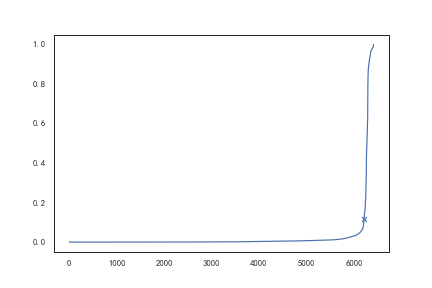
\includegraphics[width=0.9\linewidth]{./data/渤海银行.png}
	\caption{标记处为渤海银行预测点}
	\label{fig:bhyh}
\end{figure}

\section{机器学习验证与比较}
违约实际上并非线性的因素叠加,包含了非线性的因素,如华夏幸福违约,既存在过度扩张导致现金流承压,又存在重要股东拒绝为其扩张买单,最终资金链断裂。虽然可以通过加入交互项刻画这种“同时发生”的作用,但会发生“维度灾难”,可用数据变得稀疏。
机器学习适合于提取其中非线性因素。但违约样本是偏态分布的,违约债只占约 1\%,通过神经网络等方式的机器学习极有可能会欠拟合或过拟合,使机器判断有误。
综合考虑下决定采用决策树和随机森林两种受样本分布偏态影响较小的方式进行预测。
决策树是通过二叉树这一数据结构,通过最大化信息增益的手段训练分类器,比较直观且可解释性较强。而随机森林则是一种集成算法,即通过构建多棵决策树“投票”的“森林”训练器,对于不平衡的数据集来说,它可以平衡误差,但缺乏可解释性。

决策树训练结果可视化如图\ref{fig:decision_tree}所示,Logit 模型和两种机器学习算法模型准确率如表\ref{tab:acc}所示。

\begin{figure}[h]
	\centering
	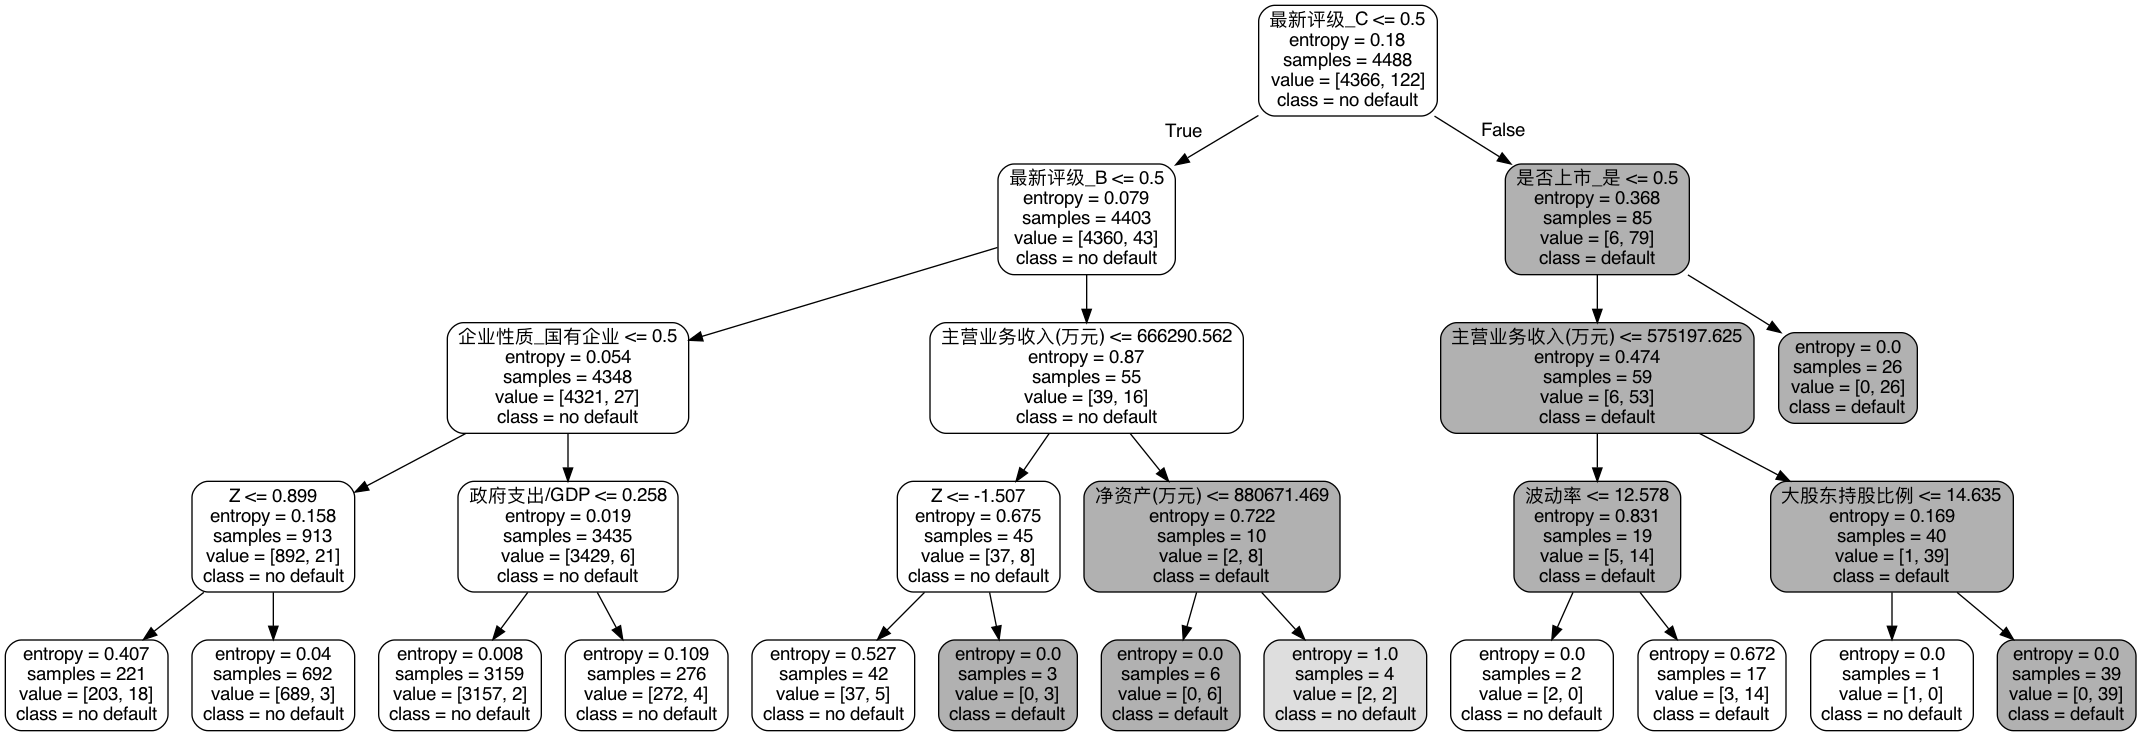
\includegraphics[width=.9\linewidth]{./data/decision_tree.png}
	\caption{\label{fig:decision_tree}决策树}
\end{figure}

图\ref{fig:decision_tree}决策树算法的关键节点如波动率、主营收入、企业性质、Z 值等在 Logit 模型中显著,在 Logit 模型中不显著的大股东持股比例分枝后判断的概率值仅勉强超过阈值,与 Logit 模型互相印证。

\begin{table}
	\caption{\label{tab:acc}不同模型的比较}
	\centering
	\begin{tabular}{lrrrrr}
		                      & accuracy & error rate & precision & recall & f1   \\
		\hline
		全部预测不违约        & 0.99     & 0.01       & -         & 0      & -    \\
		Logistic(全样本)      & 0.99     & 0.01       & 0.86      & 0.72   & 0.78 \\
		Decision Tree(测试集) & 0.99     & 0.01       & 0.93      & 0.73   & 0.82 \\
		Random Forest(测试集) & 0.99     & 0.01       & 0.85      & 0.70   & 0.76 \\
	\end{tabular}
\end{table}

表\ref{tab:acc}中准确率 accuracy 为预测正确的概率,精确率 precision 为预测违约的样本中确实违约的概率,召回率 recall 为事实违约样本中预测正确的概率。精确率和召回率是两个不同方面的分类器评价指标,他们的调和平均 F1 > 0.5 则说明该分类器是有效的。表\ref{tab:acc}中准确率与全部预测不违约的 0.99 相同,这是由于样本分布偏态造成的。但 F1 值均高于 0.5 ,证明本文使用的三个分类器都有一定的价值。且决策树算法相对优于其他算法。
决策树优于 Logit 模型算法在于其包含了非线形因素分枝。
而随机森林可能存在一定的训练集上的过拟合,因而表现出的性能较决策树更低。
如图\ref{fig:roc}所示,ROC 曲线的含义是设定任意阈值,得到的真阳性率和假阳性率。随后不断更改阈值,得到 ROC 曲线。AUC 定义为 ROC 曲线下的阈值,AUC面积越大一般认为模型拟合越好。可以看出在训练集上随机森林模型可能存在一定的过拟合,导致 AUC 达到 0.99 ,而 Logit 模型在训练集上表现不佳。
\begin{figure}[h]
	\centering
	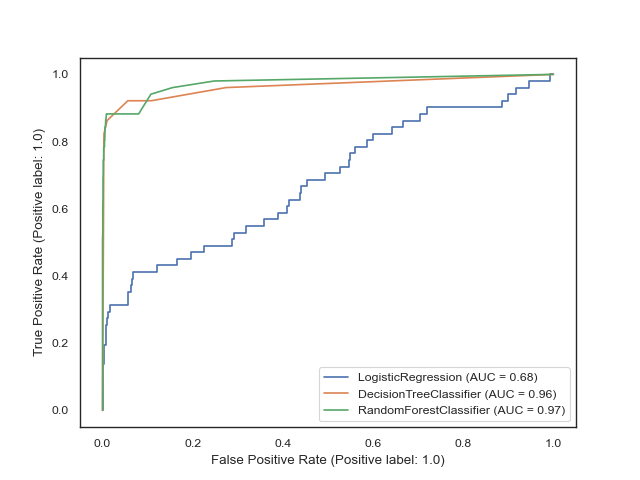
\includegraphics[width=.9\linewidth]{./data/roc.png}
	\caption{\label{fig:roc}ROC曲线与AUC值}
\end{figure}

\section{稳健性检验}
表 \ref{tab:Logitresult} 中作为财务指标的 Z 值显著。wind 数据库会直接提供 Z 值给投资者使用,其 Z 值的计算公式为
\begin{equation}
	\label{eq:1}
	Z=1.2X_1+1.4X_2+3.3X_3+0.6X_4+0.999X_5
\end{equation}
其中 \(X_1\)代表营运资本/总资产,\(X_2\)代表留存收益/总资产,\(X_3\)代表息税前利润/总资产:以上变量及 \(X_5\) 均可以直接获得一致的数据;\(X_4\)代表总市值/负债总计,而当企业非上市,总市值数据不可得时,则使用股东权益代替。

式 \ref{eq:1} 中的 \(X_{5}\) 包括了营业收入/总资产,和主营业务收入回归元存在一定的相关性。可能模型中主营业务收入非常显著,因而导致 Z 值显著,而非 Z 值本身带有一定的经济学逻辑。为检验此种可能性,本文将计算 Z 值的元素展开。如果该可能性成立,则有假设:

\begin{hyp}
	\label{hyp:1}
	展开 Z 值的回归结果 \(X_i\forall i\in [1,2,3,4] \) 应不显著,而仅仅是 \(X_5\) 显著。
\end{hyp}

\begin{center}
	\captionof{table}{稳健性检验结果\label{tab:robust}}
	\begin{tabular}{p{0.25\linewidth}p{0.2\linewidth}p{0.25\linewidth}p{0.2\linewidth}}
		\toprule
		\textbf{Dep. Variable:}   & default          & \textbf{  No. Observations:  } & 6447       \\
		\textbf{Model:}           & Probit           & \textbf{  Df Residuals:      } & 6414       \\
		\textbf{Method:}          & MLE              & \textbf{  Df Model:          } & 32         \\
		\textbf{Date:}            & Wed, 09 Mar 2022 & \textbf{  Pseudo R-squ.:     } & 0.7267     \\
		\textbf{Time:}            & 15:02:31         & \textbf{  Log-Likelihood:    } & -219.70    \\
		\textbf{converged:}       & True             & \textbf{  LL-Null:           } & -803.76    \\
		\textbf{Covariance Type:} & nonrobust        & \textbf{  LLR p-value:       } & 5.491e-225 \\
		\bottomrule
	\end{tabular}
	\begin{longtable}{p{0.18\linewidth}p{0.1\linewidth}p{0.1\linewidth}p{0.1\linewidth}p{0.1\linewidth}p{0.12\linewidth}p{0.1\linewidth}}
		\midrule
		                 & \textbf{coef} & \textbf{std err} & \textbf{z} & \textbf{P$> |$z$|$} & \textbf{[0.025} & \textbf{0.975]} \\
		\textbf{const}          & -3.8725       & 1.252            & -3.092     & 0.002               & -6.327          & -1.418          \\
		\textbf{评级\_A以上}    & -0.0382       & 0.318            & -0.120     & 0.904               & -0.661          & 0.585           \\
		\textbf{评级\_B}        & 1.4849        & 0.187            & 7.938      & 0.000               & 1.118           & 1.852           \\
		\textbf{评级\_C}        & 3.6740        & 0.228            & 16.102     & 0.000               & 3.227           & 4.121           \\
		\textbf{国有企业}       & -1.6422       & 0.398            & -4.128     & 0.000               & -2.422          & -0.862          \\
		\textbf{外资企业}       & -1.1744       & 0.467            & -2.514     & 0.012               & -2.090          & -0.259          \\
		\textbf{民营企业}       & -0.7078       & 0.385            & -1.839     & 0.066               & -1.462          & 0.046           \\
		\textbf{集体企业}       & -1.2313       & 0.534            & -2.307     & 0.021               & -2.277          & -0.185          \\
		\textbf{上市企业}       & -0.1945       & 0.192            & -1.014     & 0.310               & -0.570          & 0.181           \\
		\textbf{持有基金占比}   & -0.0783       & 0.080            & -0.973     & 0.331               & -0.236          & 0.079           \\
		\textbf{大股东持股比例} & -0.0013       & 0.003            & -0.508     & 0.611               & -0.006          & 0.004           \\
		\textbf{应付账款(万元)} & 1.409e-12     & 2.48e-12         & 0.567      & 0.570               & -3.46e-12       & 6.28e-12        \\
		\textbf{标准券折算率}   & -0.3647       & 0.651            & -0.560     & 0.575               & -1.640          & 0.911           \\
		\textbf{净资产(万元)}   & 9.314e-09     & 1.1e-08          & 0.847      & 0.397               & -1.22e-08       & 3.09e-08        \\
		\textbf{现金短债比}     & -0.1082       & 0.133            & -0.816     & 0.415               & -0.368          & 0.152           \\
		\textbf{流动性}         & -5.276e-11    & 6.63e-11         & -0.796     & 0.426               & -1.83e-10       & 7.72e-11        \\
		\textbf{政府支出/GDP}   & 1.2248        & 2.087            & 0.587      & 0.557               & -2.866          & 5.315           \\
		\textbf{SHIBOR}         & 0.3573        & 0.190            & 1.881      & 0.060               & -0.015          & 0.730           \\
		\textbf{波动率}         & 0.0341        & 0.016            & 2.135      & 0.033               & 0.003           & 0.065           \\
		\textbf{房地产政策}     & 0.7415        & 0.411            & 1.805      & 0.071               & -0.064          & 1.547           \\
		\textbf{X1}             & -0.0083       & 0.003            & -3.009     & 0.003               & -0.014          & -0.003          \\
		\textbf{X2}             & -0.0037       & 0.002            & -2.375     & 0.018               & -0.007          & -0.001          \\
		\textbf{X3}             & -0.0062       & 0.004            & -1.638     & 0.101               & -0.014          & 0.001           \\
		\textbf{X4}             & -0.0064       & 0.002            & -3.917     & 0.000               & -0.010          & -0.003          \\
		\textbf{X5}             & 0.0005        & 0.001            & 0.530      & 0.596               & -0.001          & 0.002           \\
		\bottomrule
	\end{longtable}
\end{center}

回归结果如表
\ref{tab:robust}
所示,与表 \ref{tab:Logitresult} 相比基本一致,仅 SHIBOR 利率变为显著,且\(X_1\) 至 \(X_4\) 均显著,说明 Z 值中的其他成分均具有一定的预测能力,而非只是受到主营收入的影响导致显著,假设 H\ref{hyp:1}不成立。
